% !TEX root = ../00_thesis.tex

\section{Appendix -- MILP Formulation}
\label{appendix:single_mode}

\TODO{read carefully (will need to be adapted to the new sched synthesis) and potential merge with the tech report version}

This appendix presents the complete description of the ILP formulation, used to synthesize the schedule \sched{\mode{}} of a given operation mode \mode{}, \ie
\begin{align*}
&\sched{\mode{}} \; = \;
	\left\lbrace
	\begin{tabular}{c@{\quad}|@{\quad}l}
	$\tau.o, \, m.o, \, m.d$
	&
	$\app \in \mode{}, \;
	(\tau,m) \in \app.\predG$
	\\
	$r_k.t, \, r_k.[B]$
	&
	$k \in [1, \, R_{\mode{}}]$
	\end{tabular}
	\right\rbrace
\end{align*}


The system model is described in \cref{sec:model}. All the variables and parameters involved in the ILP formulation used to solve the single-mode schedule synthesis problem are listed at the end in Table~\ref{tab:ILPvar} for reference.
This appendix details all the formulated constraints and how they are implemented in practice. The last subsection details the formulation of the objective function used to minimize the end-to-end application latency.

%%1. Pseudo-code that shows how we guarantee that the number of rounds is minimized
%The schedule of a mode \mode{} is computed for one hyperperiod, after which it repeat itself.
%To minimize the number of rounds used, we solve the problem sequentially, as described in Alg.~\ref{alg:outerlayer}.
%Each ILP formulation considers a fixed number of rounds $R_{\mode{}}$ to be scheduled, starting with $R_{\mode{}}=0$. The number of rounds is incremented until a feasible solution is found, or until the maximum number of rounds $R_{max}$ -- the number of rounds that ``fit'' into one hyperperiod -- is reached.
%Thus, Alg.~\ref{alg:outerlayer} guarantees by construction that if the problem is feasible, the synthesized schedule is optimal in terms of number of rounds used.
%The end-to-end latency is minimized by setting the sum of all application's latency as objective function.
%
%
%\begin{algorithm}
%\begin{algorithmic}
%\small
%\Require
%	mode \mode{},
%	applications $\app \in \mode{}$,
%	task mappings $\tau.map$ and WCETs $\tau.e$,
%	round duration $\Tround$
%	\; -- \;
%\textbf{Output:}
%	\sched{M}
%
%\State $LCM \gets$ \textit{hyperperiod}(\mode{})
%%\State $R_{min} = 1$
%\State $R_{max} = floor(LCM/\Tround)$
%
%\State $R_{\mode{}} = 0$
%
%\While{$R_{\mode{}} \leq R_{max}$}
%	\State formulate the ILP for mode \mode{} using $R_{\mode{}}$ rounds
%%	ILP = \textit{pbmFormulation}( \mode{} , $R$ )
%	\State [ \sched{M}, \textit{feasible} ] = \textit{solve}( ILP )
%	\If {\textit{feasible}}
%		\Return \sched{M}
%	\EndIf
%	\State $R_{\mode{}} \gets R_{\mode{}}+1$
%\EndWhile
%\State \Return 'Problem unfeasible'
%\end{algorithmic}
%\caption{Pseudo-code of the schedule synthesis}
%\label{alg:outerlayer}
%\end{algorithm}


The ILP formulation to be solved by Alg.~\ref{alg:outerlayer} (see \cref{sec:model}) contains the following constraints, which can be classified into four categories.

\fakepar{1. Application constraints}
		\begin{description}
			\item[(C1.1)] Precedence constraints between tasks and messages must be respected.
			\item[(C1.2)] End-to-end deadlines must be satisfied.
		\end{description}

\fakepar{2. Round constraints}
		\begin{description}
			\item[(C2.1)] The rounds must not be overlapping.
			\item[(C2.2)] The time interval between two rounds is upper-bounded.
		\end{description}

\fakepar{3. Validity of the tasks mapping}
		\begin{description}
			\item[(C3)] The same node cannot process more than one task simultaneously.
		\end{description}

\fakepar{4. Validity of the messages allocation}
		\begin{description}
			\item[(C4.1)] Every message must be served
			after its release time.
			\item[(C4.2)] Every message must be served
			before its deadline.
			\item[(C4.3)] A round cannot be allocated more messages than the number of slots available in one round.
			\item[(C4.4)] Within one hyperperiod, the same number of messages are released and served.
		\end{description}

The validity of the message allocation constraints, in particular constraints \textbf{(C4.1)} and \textbf{(C4.2)}, induce a non-linear coupling between the message and round variables. This peculiar aspect makes the scheduling problem non-trivial and prevents the use of conventional ILP-based schedule synthesis approaches reported thus far in the literature.
Our approach to solve this problem is detailed in \cref{sec:message_alloc}.


\subsection*{Application constraints}\label{sec;application}
\begin{description}
	\item[(C1.1)]Precedence constraints between tasks and messages must be respected.
\end{description}
For any application \app, let $\app.c$ be a \emph{chain} in \app.\predG. A chain is a path of \app.\predG starting and ending with a task without predecessor and successor, respectively. $\app.c(\,\first\,)$ and $\app.c(\,\last\,)$ denote the first and last task of the chain \app.c.  $\sigma_{i,j}$ is a binary variable accounting for the cases where successive task $\tau_i$ and message $m_j$ (resp. a message $m_i$ and task $\tau_j$) start during different application period ($\sigma_{i,j} = 1$) or not ($\sigma_{i,j} = 0$)
\begin{align}
\intertext{%
$	\forall\, \app, \;
	\forall\, \app.c \in \app.\predG, \;
	\forall\, \tau_j \in (\app.c \setminus \app.c(\,\last)),\;
	\forall\, m_i \in \tau_j.prec,
	$}
		m_i.o + m_i.d
		&\;\leq\; \app.p * \sigma_{i,j} + \tau_j.o\\
\intertext{%
$	\forall\, \app, \;
	\forall\, \app.c \in \app.\predG, \;
	\forall\, m_j \in \app.c,\;
	\forall\, \tau_i \in m_j.prec,
	$}
		\tau_i.o + \tau_i.e
		&\;\leq\; \app.p * \sigma_{i,j} + m_j.o
\end{align}

\begin{description}
	\item[(C1.2)] End-to-end deadlines must be satisfied.
\end{description}
\begin{align}
\intertext{%
$	\forall\, \app, \;
	\forall\, \app.c \in \app.\predG, \;
		\tau_{\first} = \app.c(\,\first\,), \;
		\tau_{\last} = \app.c(\,\last\,), \;
		C = |\app.c|, $}
& \tau_{\last}.o + \tau_{\last}.e - \tau_{\first}.o + \sum_{j=1}^{C-1} \app.p*\sigma_{i,j}  \;\leq\; \app.d
\end{align}



\subsection*{Round constraints}\label{sec:rounds}
\begin{description}
	\item[(C2.1)]The rounds must not be overlapping.
\end{description}
\begin{flalign}
&\forall j \in [1..R_{\mode{}}-1],
& & r_j.t + \Tround \; \leq \; r_{j+1}.t
&
\end{flalign}

\begin{description}
	\item[(C2.2)]The time interval between two rounds is upper-bounded.
\end{description}
%\begin{align}
%\intertext{%
%$	\forall j \in [1..R_{\mode{}}-1],$}
%&r_{j+1}.t - r_j.t  \; \leq \;  T_{max}
%\end{align}
\begin{flalign}
&\forall j \in [1..R_{\mode{}}-1],
&
&r_{j+1}.t - r_j.t  \; \leq \;  T_{max}
&
&
\end{flalign}


\subsection*{Validity of the task mappings}\label{sec:task_mapping}
\begin{description}
	\item[(C3)]The same node cannot process more than one task simultaneously.
\end{description}
\begin{align}
\intertext{%
$	\forall\, \tau_i, \tau_j, \; \tau_i.map == \tau_j.map, \;
	\forall\, k_i \in [1..LCM/\tau_i.p], \; \forall\, k_j \in [1..LCM/\tau_j.p]$}
\label{eq:t1beforet2}
&	\tau_i.o + \tau_i.e + \tau_i.p*k_i \; \leq \; \tau_j.o + \tau_j.p*k_j \\
\label{eq:t2beforet1}
\texttt{or} \quad
&	\tau_j.o + \tau_j.e + \tau_j.p*k_j \; \leq \; \tau_i.o + \tau_i.p*k_i
\end{align}
%
However, an ILP formulation cannot directly support that only one-out-of-two constraints must be satisfied. To resolve this, we use a classical trick using $(i)$ a binary variable $\lambda$ representing which of the two constraints \eqref{eq:t1beforet2} or \eqref{eq:t2beforet1} must be enforced and $(ii)$ a ``big'' time constant $M$, used to satisfied the other constraint by default, \ie regardless of the values of the variables. For example, $M = 10*LCM$.
%
\begin{align}
\label{eq:t1beforet2_impl}
\tau_i.o + \tau_i.e + \tau_i.p*k_i
	&\; \leq \; \tau_j.o + \tau_j.p*k_j + M\!M * (1 - \lambda_{i,j}^{k_i,k_j}) \\
\label{eq:t2beforet1_impl}
\tau_j.o + \tau_j.e + \tau_j.p*k_j
	&\; \leq \; \tau_i.o + \tau_i.p*k_i + M\!M * \lambda_{i,j}^{k_i,k_j}
\end{align}
%
With this implementation of the constraints, it follows that
%
\begin{align*}
&	\lambda_{i,j}^{k_i,k_j} = 1
	\quad \Leftrightarrow \quad
		\eqref{eq:t1beforet2_impl} \equiv \eqref{eq:t1beforet2}
%		\; and \;
		\;\wedge\;
		\eqref{eq:t2beforet1_impl} \text{ is always satisfied.}
		\\
&	\lambda_{i,j}^{k_i,k_j} = 0
	\quad \Leftrightarrow \quad
		\eqref{eq:t2beforet1_impl} \equiv \eqref{eq:t2beforet1}
% 		\; and \;
		\;\wedge\;
		\eqref{eq:t1beforet2_impl} \text{ is always satisfied.}
\end{align*}






\subsection*{Validity of the messages allocation}\label{sec:message_alloc}

As mentioned earlier, the validity of the message allocation constraints, in particular constraints \textbf{(C4.1)} and \textbf{(C4.2)}, induce a non-linear coupling between the message and round variables. This peculiar aspect makes the scheduling problem non-trivial and prevents the use of conventional ILP-based schedule synthesis approaches reported thus far in the literature.
The following subsection repeats and deepens the arguments from \cref{sec:single_mode}.

%-> Formulate constraints based on Network Calculus: arrival, service and demand functions
To address problem of variable coupling, we first formulate the constraints \textbf{(C4.1)} and \textbf{(C4.2)} using \emph{arrival}, \emph{demand}, and \emph{service} functions, \af \df and \sf, using network calculus%
%~\cite{leboudec2001network}
. Those functions count the number of message instances released, served, and due since the beginning of the hyperperiod, respectively.
Those three functions are illustrated in \cref{fig:afdfsf2}.
It must hold that
\begin{flalign}
\label{eq:df<sf<af2}
&\forall\, m_i \in \messageset, \;\forall\, t,
&&\df_i(t) \leq \sf_i(t) \leq \af_i(t)
&&\\
\label{eq:af_def2}
&\text{with},
&&\af_i: \; t \;
	\longmapsto \; \left \lfloor{\frac{t-m_i.o}{m_i.p}}\right \rfloor 	+ 1
	&&\\
\label{eq:df_def2}
&\text{and},
&&\df_i: \; t \;
	\longmapsto \; \left \lceil{\frac{t-m_i.o-m_i.d}{m_i.p}}\right \rceil
	&&
\end{flalign}

\noindent
%-> Adapt them to the use of rounds
%In general, one must verify that \eqref{eq:df<sf<af} holds true for all time.
However, as the service function stays constant between the rounds, we can formulate \textbf{(C4.1)} and \textbf{(C4.2)} as follows\\
$\forall\, m_i \in \messageset, \; \forall\, j \in [1 .. R_{\mode{}}], $
\begin{flalign}
\label{eq:af_const2}
&\textbf{(C4.1)}  : \quad
	&\sf_i(r_j.t + \Tround) \, &\leq \, \af_i(r_j.t)&&
\\
\label{eq:df_const2}
&\textbf{(C4.2)}  : \quad
	&\sf_i(r_j.t)  \, &\geq \, \df_i(r_j.t + \Tround)&&
\end{flalign}

\begin{figure}
\centering
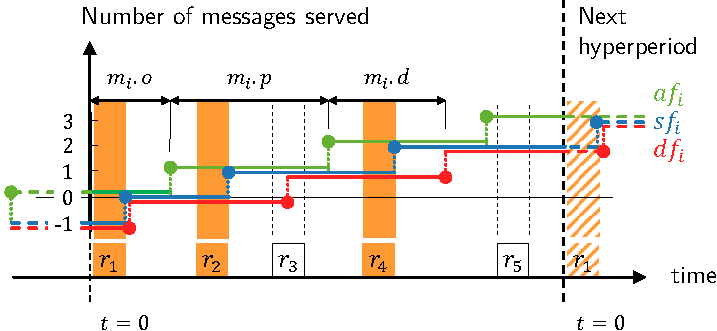
\includegraphics[scale=1]{afdfsf}
\caption{Representation of arrival, demand, and service functions of message $m_i$.
The lower part shows the five round, $r_1$ to $r_5$, scheduled for the hyperperiod.
\capt{%
$m_i$ is allocated a slot in the colored rounds, \ie $r_1$, $r_2$, and $r_4$.
The allocation of $m_i$ to $r_3$ instead of $r_2$ would be invalid, as $r_3$ does not finish before the message deadline, \ie it violates \textbf{(C4.2)}.
However, the allocation of $m_i$ to $r_5$ instead of $r_1$ would be valid and result in $r_0.B_i = 0$.}
}
\label{fig:afdfsf2}
\end{figure}


%-> Introduce integer variables constrained to match the values of \af and \df at time points of interest
\noindent
The arrival and demand functions are step functions. They cannot be used directly in an ILP formulation, however
\begin{flalign}
\label{eq:af=k2}
&\forall \; k \in \mathbb{N}, \quad
&&\af_i(t) = k
	\quad \Leftrightarrow \quad
	0 \, \leq \, t - m_i.o - (k-1)m_i.p \,<\, m_i.p &&\\
&\text{and} %\hspace{30pt}
&&\df_i(t) = k
\label{eq:df=k2}
	\quad \Leftrightarrow \quad
	0 \, < \, t - m_i.o - m_i.d - (k-1)m_i.p \,\leq\, m_i.p &&
\end{flalign}
% We introduce a set of integer variable k^a_{ij} k^d such that
For each message $m_i\in \messageset$ and each round $r_j$, $j \in [1..R_{\mode{}}]$, we introduce two integer variables $k^a_{ij}$ and $k^d_{ij}$ that we constraint to take the values of \af and \df at the time points of interest, \ie $r_j.t$ and $r_j.t + \Tround$ respectively. That is,
\begin{align}
\label{eq:ka2} %\qquad
0 \, \leq \, r_j.t
	&-m_i.o - (k^a_{ij}-1)m_i.p \,<\, m_i.p\\
\label{eq:kd2} %\qquad
0 \, < \, r_j.t
	&+\Tround - m_i.o - m_i.d - (k^d_{ij}-1)m_i.p \,\leq\, m_i.p\\
\notag
\text{Thus,} \hspace{15pt} &\eqref{eq:ka2} \quad \Leftrightarrow  \quad
	 \af_i(r_j.t) = k^a_{ij} \\
\notag
	&\eqref{eq:kd2} \quad \Leftrightarrow \quad
	\df_i(r_j.t + \Tround) = k^d_{ij}
\end{align}

%
%-> Express \sf based on the rounds

\TODO{Here might be the place to say something about the round atomicity...}
Finally, we must express the service function \sf, which counts the number of message instances served \emph{at the end} of each round.
Remember that $r_k.B_s$ denotes the allocation of the $s$-{th} slot of $r_k$.
For any time $t \in \; [ \; r_{j} + \Tround \, ; \,  r_{j+1} + \Tround \; [$, the number of instances of message $m_i$ served is
\begin{align*}
	\sum_{\substack{k = 1}}^{j}
	\sum_{\substack{s = 1}}^{B}
	 \; r_k.B_s
	 \quad s.t. \; B_s = i
\end{align*}

\noindent
It may be that $m.o + m.d > m.p$, resulting in $\df(0)=-1$ (see \eqref{eq:df_def2}), like \eg in \cref{fig:afdfsf2}. This ``means'' that a message released at the each of one hyperperiod will have its deadline in the \emph{next} hyperperiod.
To consider this situation, we introduce, for each message $m_i$, a variable $r_0.B_i$ set to the number of such ``leftover'' message instances at $t=0$.
The system model makes the assumption that $\app.d \leq \app.p$. As $m.p = \app.p$, $m.o \leq m.p$ and $m.d < \app.d$, then $m.o + m.d < 2*m.p$. Thus, there can be only one or zero of such leftover message instances, \ie $r_0.B_i \in \{0\,,\,1\}$.
Finally, for each message $m_i \in \messageset$, and  $t \in \; [ \; r_{j} + \Tround \, ; \,  r_{j+1} + \Tround \; [$,
%
%However, it may be that the last message released during one hyperperiod has its relative deadline in the \emph{next} hyperperiod, thus yielding $df(0)=-1$. It is the case \eg in \cref{fig:afdfsf}. Then, to account for this previously arrived message -- possibly not yet served -- we introduce for each message $m_i$ a variable $r_0.B_i$ set to the value of the service function $sf_i$ of message $m_i$ at $t=0$, that is $0$ or $1$. Thus finally, for each message $m_i \in \messageset$, and  $t \in \; [ \; r_{j} + \Tround \, ; \,  r_{j+1} + \Tround \; [$,
\begin{flalign}
\label{eq:sf_def2}
\sf_i: \; t \;
	&\longmapsto \;
	\sum_{\substack{k = 1 \\[2pt]s.t. \; r_k + \Tround \, < \, t}}^{j}\;\;
	\sum_{\substack{s = 1 \\[2pt]s.t. \; B_s = i}}^{B}
	 r_k.B_s - r_0.B_i
\end{flalign}

\noindent
Ultimately, \textbf{(C4.1)} and \textbf{(C4.2)} can be formulated as ILP constraints using the following four equations:
\begin{flalign}
\notag
\forall\, m_i \in \messageset, \; \forall\, j\in [1..R],
&&&\eqref{eq:ka2}\quad \;	 : \;
	\quad
	0 \, \leq \, r_j.t - m_i.o - (k^a_{ij}-1)*m_i.p \,<\, m_i.p
&&\\
\notag
&&&\eqref{eq:kd2}\quad	\; : \;
	\quad
	0 \, \leq \, r_j.t + \Tround - m_i.o - m_i.d - (k^d_{ij}-1)*m_i.p \,<\, m_i.p
&&\\
&&&\eqref{eq:af_const2}\quad	 \Leftrightarrow
	\quad
	\sum_{k = 1}^j
	\sum_{\substack{s = 1 \\[2pt]s.t. \; B_s = i}}^{B}
	 \; r_k.B_s - r_0.B_i \; \leq\;  k^a_{ij}
&&\\
&&&\eqref{eq:df_const2}\quad	 \Leftrightarrow
	\quad
	\sum_{k = 1}^{j-1}
	\sum_{\substack{s = 1 \\[2pt]s.t. \; B_s = i}}^{B} \; r_k.B_s - r_0.B_i
	\; \geq\;
	k^d_{ij}
&&
\end{flalign}

To implement those constraints in practice, some slight modifications are still required. We use Gurobi to solve the ILP problem. This solver does not allow to model strict inequalities, \ie $A \cdot x  < B$. Therefore, to implement the right-hand side of the constraints \eqref{eq:ka} and \eqref{eq:kd2}, we need to use a ``small'' time constant $mm$.
%
Furthermore,
%
This leads to the following implementation.

\begin{description}
	\item[(C4.1)]Every message must be served after its release time.
\end{description}
\begin{flalign}
&\forall\, m_i\in \messageset, \; \forall\, j\in [1..R_{\mode{}}],
\label{eq:serveAfterArrival}
&	&0  \; \leq \; r_j.t - m_i.o - (k^a_{ij}-1)*m_i.p
		\; \leq \; m_i.p - mm
&		\\
&
&	&\sum_{k = 1}^{j}
	\sum_{\substack{s = 1 \\[2pt]s.t. \; B_s = i}}^{B} \; r_k.B_s - r_0.B_i
	\; \geq\;
	k^d_{ij}
&
\intertext{%
\begin{description}
	\item[(C4.2)]Every message must be served before its deadline.
\end{description}
}
&\forall\, m_i\in \messageset, \; \forall\, j\in [1..R_{\mode{}}],
&	&mm  \; \leq \; r_j.t + \Tround - m_i.o - m_i.d - (k^d_{ij}-1)*m_i.p
		\; \leq \; m_i.p
&		\\
&
&	&\sum_{k = 1}^{j-1}
	\sum_{\substack{s = 1 \\[2pt]s.t. \; B_s = i}}^{B} \; r_k.B_s - r_0.B_i
	\; \geq\;
	k^d_{ij}
&
\end{flalign}

Finally, the formulation of the last two constraints -- \textbf{(C4.3)} and \textbf{(C4.4)} -- is rather straightforward.

\begin{description}
	\item[(C4.3)]A round cannot be allocated more messages than the number of slots available in one round.
\end{description}
%
\begin{align*}
\text{Satisfied by construction.}
\end{align*}


\begin{description}
	\item[(C4.4)] Within one hyperperiod, the same number of messages are released and served.
\end{description}
\begin{flalign}
&\forall\, m_i\in \messageset,
&
	&\sum_{k = 1}^{R_{\mode{}}}
	\sum_{\substack{s = 1 \\[2pt]s.t. \; B_s = i}}^{B} \; r_k.B_s
	\; = \; LCM/m_i.p
&&
\end{flalign}

\subsection*{Objective function}

To obtain a valid schedule, the ILP solver does not \emph{need} to optimize any objective function. The primer objective is to minimize of the number of rounds $R_{\mode{}}$ used in the schedule, which is achieved by incrementally increasing the number of rounds (see Algorithm~\ref{alg:outerlayer}) until a valid schedule is found.

However, from the application perspective, it is of importance to \emph{minimize the end-to-end latency} of concurrently running applications. Therefore, we formulate as an objective function, denoted \obj, the sum of all application latency, which we want to minimize. If we denote the latency of application \app by $\app.\delta$ and the latency of the chain $\app.c$ by $\app.c.\delta$,
\begin{align}
\intertext{%
$	\forall\, \app, \;
	\forall\, \app.c \in \app.\predG, \;
		\tau_{\first} = \app.c(\,\first\,), \;
		\tau_{\last} = \app.c(\,\last\,), \;
		C = |\app.c|, $}
\app.c.\delta \; & = \;
%	\max
%		\left(
			\tau_{\last}.o + \tau_{\last}.e - \tau_{\first}.o + \sum_{j=1}^{C-1} \app.p*				\sigma_{i,j}
%		\right)
\\
 \app.\delta \; &= \;
	\max_{\app.c \,\in\, \app.\predG}
		\left(
			\;
			\app.c.\delta
			\;
		\right)
\intertext{%
And finally,}
\obj \; &= \; \sum_{\app \,\in\, \text{mode }\mode{}} \;
	\app.\delta
\end{align}


\begin{table}[h]
\centering
\small
\caption{Complete list of variables used in the ILP formulation.}
\label{tab:ILPvar}
\input{\ChapPath/Tables/table_ILPvar.txt}
\end{table}
